\section{Case Study A: OpenCL Heterogeneous Mapping}
\label{sec:deeptune-case-study-a}

OpenCL provides a platform-agnostic framework for heterogeneous parallelism. This allows a program written in OpenCL to execute transparently across a range of different devices, from CPUs to GPUs and FPGAs. Given a program and a choice of execution devices, the question then is on which device should one execute the program to maximise performance?

\subsection{State-of-the-art}

We return to the \citeauthor{Grewe2013}~\cite{Grewe2013} predictive model for mapping OpenCL kernels to the optimal device in CPU/GPU heterogeneous systems, previously used in Chapter~\ref{chap:clgen}. They use supervised learning to construct decision trees, using a combination of static and dynamic kernel features. The static program features are extracted using a custom LLVM pass; the dynamic features are taken from the OpenCL runtime.

\paragraph*{Expert Chosen Features}

Table~\ref{tab:grewe-features-final} shows the features used in their work. Each feature is an expression built upon the code and runtime metrics given in Table~\ref{tab:grewe-features-raw}.

\begin{table}
  \rowcolors{2}{gray!25}{white}
  \centering%
  \subfloat[Feature values]{
    \begin{tabular}{| l L{4.5cm} |}
      \hline
      \rowcolor{gray!50}
      \textbf{Name} & \textbf{Description} \\
      \hline
      \texttt{F1: data size/(comp+mem)} & commun.-computation ratio \\
      \texttt{F2: coalesced/mem} & \% coalesced memory accesses \\
      \texttt{F3: (localmem/mem)$\times$wgsize} & ratio local to global mem accesses  $\times$ \#.\ work-items \\
      \texttt{F4: comp/mem} & computation-mem ratio\\
      \hline
    \end{tabular}%
    \label{tab:grewe-features-final}%
  }\\ %
  \subfloat[Values used in feature computation]{%
    \rowcolors{2}{gray!25}{white}
    \begin{tabular}{| l c l |}
    	\hline
      \rowcolor{gray!50}
      \textbf{Name} & \textbf{Type} & \textbf{Description} \\
      \hline
      \texttt{comp} & static & \#.\ compute operations \\
      \texttt{mem} & static & \#.\ accesses to global memory \\
      \texttt{localmem} & static & \#.\ accesses to local memory \\
      \texttt{coalesced} & static & \#.\ coalesced memory accesses \\
      \texttt{data size} & dynamic & size of data transfers \\
      \texttt{work-group size} & dynamic & \#.\ work-items per kernel \\
      \hline
    \end{tabular}%
    \label{tab:grewe-features-raw}%
  }
  \caption[Heterogeneous mapping model features]{%
    Features used by \emph{Grewe et al. }to predict heterogeneous device
    mappings for OpenCL kernels.%
  } %
  \label{tab:grewe-features} %
\end{table}


\subsection{Experimental Setup}

The predictive model of \citeauthor{Grewe2013}~\cite{Grewe2013} is replicated. The same experimental setup is used as in Chapter~\ref{chap:clgen} in which the experiments are extended to a larger set of 71 programs, summarised in Table~\ref{tab:cgo-benchmarks}. The programs were evaluated on two CPU-GPU platforms, detailed in Table~\ref{tab:cgo-platforms}.

\begin{table}
  \centering%
  \rowcolors{2}{gray!25}{white}
  \begin{tabular}{| l r r r |}
    \hline
    \rowcolor{gray!50}
    & \textbf{Version} & \textbf{\#. benchmarks} & \textbf{\#. kernels}\\
    \hline
    \textbf{NPB (SNU~\cite{Seo2011})} & 1.0.3 & 7 & 114 \\
    \textbf{Rodinia~\cite{Che2009}} & 3.1 & 14 & 31 \\
    \textbf{NVIDIA SDK} & 4.2 & 6 & 12 \\
    \textbf{AMD SDK} & 3.0 & 12 & 16 \\
    \textbf{Parboil~\cite{Stratton2012}} & 0.2 & 6 & 8 \\
    \textbf{PolyBench~\cite{Grauer-Gray2012}} & 1.0 & 14 & 27 \\
    \textbf{SHOC~\cite{Danalis2010}} & 1.1.5 & 12 & 48 \\
    \textbf{Total} & - & 71 & 256 \\
    \hline
  \end{tabular}
  \caption[Benchmarks used in Case Study A]{%
    Benchmarks used in Case Study A.%
  }
  \label{tab:cgo-benchmarks}
\end{table}

\begin{table}[t!]
  \centering %
    \rowcolors{2}{gray!25}{white}
    \begin{tabular}{| l l l l| }
      \hline
      \rowcolor{gray!50}
      & \textbf{Frequency} & \textbf{Memory} & \textbf{Driver} \\
      \hline
      \textbf{Intel Core i7-3820} & 3.6 GHz & 8GB & AMD 1526.3 \\
      \textbf{AMD Tahiti 7970} & 1000 MHz & 3GB & AMD 1526.3 \\
      \textbf{NVIDIA GTX 970} & 1050 MHz & 4GB & NVIDIA 361.42 \\
      \hline
    \end{tabular}
    \caption[Benchmarks used in Case Study A]{%
    Experimental platforms used in Case Study A.%
    }
    \label{tab:cgo-platforms}
\end{table}


\paragraph*{DeepTune Configuration}

Figure~\ref{fig:nn}a shows the neural network configuration of DeepTune for the task of predicting optimal device mapping. The OpenCL kernel source code is used as input, along with the two dynamic values \emph{work-group size} and \emph{data size} available to the OpenCL runtime.

\paragraph*{Model Evaluation}

\emph{Stratified 10-fold cross-validation} is used to evaluate the quality of the predictive models~\cite{Han2011}. Each program is randomly allocated into one of 10 equally-sized sets; the sets are balanced to maintain a distribution of instances from each class consistent with the full set. A model is trained on the programs from all but one of the sets, then tested on the programs of the unseen set. This process is repeated for each of the 10 sets, to construct a complete prediction over the whole data set.

\begin{figure}[t!]
  \centering
  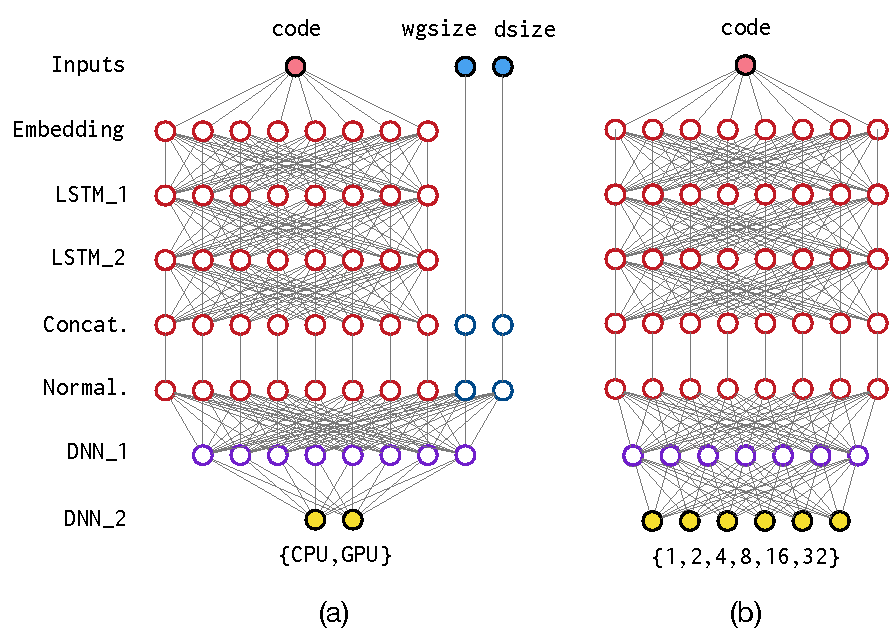
\includegraphics[width=\columnwidth]{img/nn} %
  \caption[DeepTune artificial neural networks]{%
    DeepTune artificial neural networks, configured for (a) heterogeneous mapping, and (b) thread coarsening factor. The design stays almost the same regardless of the optimisation problem. The only changes are the extra input for (a) and size of the output layers.%
  }%
  \label{fig:nn}
\end{figure}



\subsection{Experimental Results}

Selecting the optimal execution device for OpenCL kernels is essential for maximising performance. For a CPU/GPU heterogeneous system, this presents a binary choice. In this experiment, the approach is compared against a static single-device approach and the \citeauthor{Grewe2013} predictive model. The \emph{static mapping} selects the device which gave the best average case performance over all the programs. On the AMD platform, the best-performing device is the CPU; on the NVIDIA platform, it is the GPU.

Figure~\ref{fig:cgo-accuracy} shows the accuracy of both predictive models and the static mapping approach for each of the benchmark suites. The static approach is accurate for only 58.8\% of cases on AMD and 56.9\% on NVIDIA. This suggests the need for choosing the execution device on a per program basis. The \citeauthor{Grewe2013} model achieves an average accuracy of 73\%, a significant improvement over the static mapping. By automatically extracting useful feature representations from the source code, DeepTune gives an average accuracy of 82\%, an improvement over both schemes.

\begin{figure}
  \centering %
  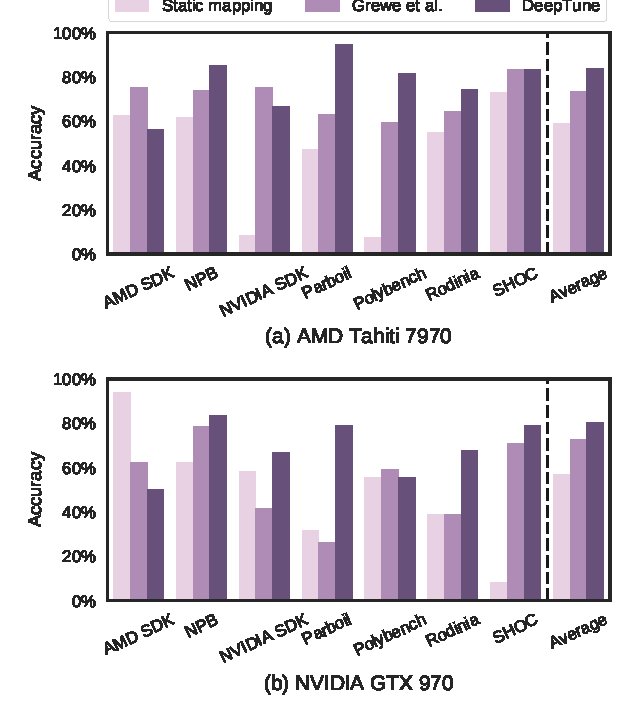
\includegraphics[width=.85\columnwidth]{img/cgo-acc}%
  \caption[Accuracy of optimisation heuristics for heterogeneous device mapping]{%
    Accuracy of optimisation heuristics for heterogeneous device mapping, aggregated by benchmark suite. The optimal static mapping achieves 58\% accuracy. The \citeauthor{Grewe2013} and DeepTune predictive models achieve accuracies of 73\% and 84\%, respectively.%
  }
  \label{fig:cgo-accuracy}
\end{figure}

Using the static mapping as a baseline, the relative performance of each program is computed using the device selected by the \citeauthor{Grewe2013} and DeepTune models. Figure~\ref{fig:cgo-speedup} shows these speedups. Both predictive models significantly outperform the static mapping; the Grewe \emph{et al.\ }model achieves an average speedup of $2.91\times$ on AMD and $1.26\times$ on NVIDIA (geometric mean $1.18\times$). In 90\% of cases, DeepTune matches or outperforms the predictions of the Grewe \emph{et al.\ }model, achieving an average speedup of $3.34\times$ on AMD and $1.41\times$ on NVIDIA (geometric mean $1.31\times$). This 14\% improvement in performance comes at a greatly reduced cost, requiring no intervention by humans.

\begin{figure}
  \centering %
  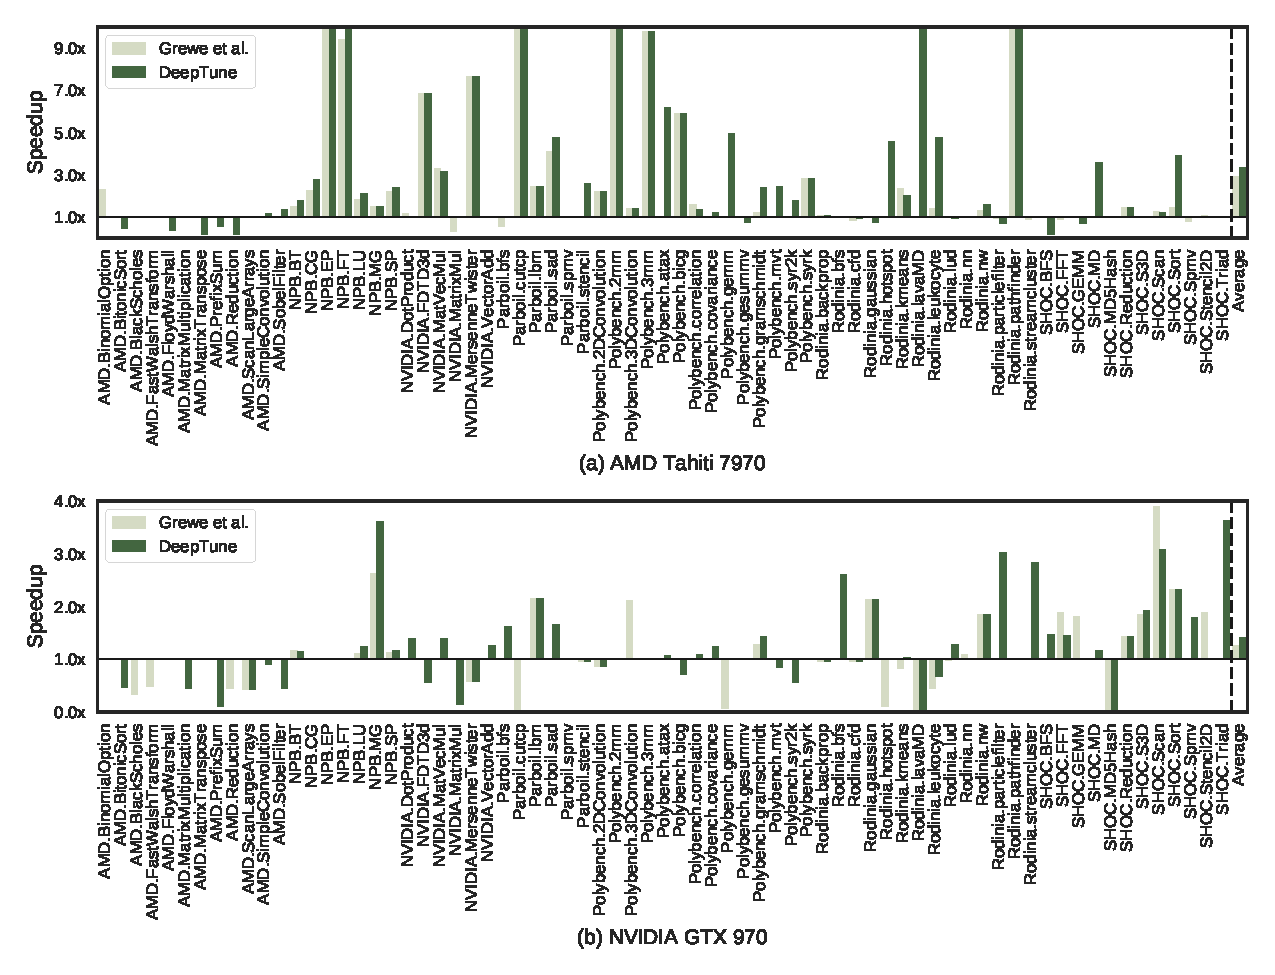
\includegraphics[width=\textwidth]{img/cgo-speedup}%
  \caption[Speedup of predicted heterogeneous mappings]{%
    Speedup of predicted heterogeneous mappings over the best static mapping for both platforms. In (a) DeepTune achieves an average speedup of 3.43x over static mapping and 18\% over \citeauthor{Grewe2013}. In (b) the speedup is 1.42x and 13\% respectively.%
  }
  \label{fig:cgo-speedup}
\end{figure}
